\documentclass[12pt] {article}
\usepackage{times}
\usepackage[margin=0.7in,bottom=1in,top=0.5in]{geometry}

\usepackage{hhline}
\usepackage{subfig}
\usepackage{amsmath}
\usepackage{amsfonts}
\usepackage[inline,shortlabels]{enumitem}%enumerate with letters
\usepackage{mathrsfs} 
\usepackage[square,numbers]{natbib}
\usepackage{graphicx}
\usepackage{natbib}
\usepackage{color}
\usepackage[mathscr]{euscript}
\usepackage{wrapfig}
\usepackage{hyperref}
\begin{document}
\bibliographystyle{apalike}
\title{
Final Project -  EEC254 \\
\begin{large}
Floor Planning via Convex Optimization
\end{large}
}
\author{Ahmed Mahmoud}
\date{}
\maketitle

%============Table========
%\begin{figure}[tbh]
% \centering    
%\begin{tabular}{ |p{4cm}|| p{2cm}|p{2cm}|p{2cm}|p{2cm}|}
% \hline
% & Processor 1 &  Processor 2  & Processor 3 & Processor 4\\ \hhline{|=|=|=|=|=|}
% \hline
% Performance          &$1.08$        &$1.425$       &\textbf{1.52}  &   \\
% \hline
%\end{tabular} 
%\caption{Metric table for the four processors}
%   \label{tab:metric}
%\end{figure} 
%============Figure========
%\begin{figure}[!tbh]
%\centering        
%   \subfloat {\includegraphics[width=0.65\textwidth]{fig2_4.png}}
%   \caption{ }
%   \label{fig:fig}
%\end{figure}

%\begin{enumerate}[(a)]
%\end{enumerate}

%\section{Abstract}
%===========================================
\section{Introduction}
Floor planning problem tries to find the optimal position and/or dimensions of geometric objects (commonly rectangles) within a space such that there is no overlap between them. We refer to the objects as \emph{cells} which are axis-aligned. There could be some constraints on the cells e.g., area-constraints, aspect ratio constraints, and positions constraints. The objective is usually to minimize the size (e.g., area, volume, perimeter) of the bounding rectangle or maximize the size of the cells.

%===========================================
\section{System Model}
We consider $N$ axis-aligned cells ($c_{1}, \cdots, c_{N}$) in 2D each specified by its lower-left corner $(x_{i}, y_{i})$, height $h_{i}$, and width $w_{i}$. The cells are configured inside a bounding rectangle (BR) of height $H$, width $W$, and the origin as its lower-left corner. The cells are always desired to not overlap. This constraint makes the general floor-planning a complicated combinatorial optimization problem. However, if the relative positioning of the cells is specified, the floor-planning problem can be cast as convex optimization. 
\subsection*{Variables}
The variables of the optimization problem are the position and size of the cells ($x_{i}, y_{i}, h_{i}, w_{i}$ for $i=1,\cdots, N$) and the size of the bounding rectangle ($H$, $W$). 
\subsection*{Objectives} 
There are two different objectives that the problem of floor-planning may try to achieve either of them 
\begin{enumerate}
\item Minimizing the are of the bounding rectangle of fixed-size cells. Here we consider minimizing the perimeter of the bounding rectangle since the area is a non-convex function and its log is concave function.
\item Maximizing the area of the cells for a fixed-size bounding rectangle. We take log are of the cell i.e., $max (log(w_{i})+log(h_{i}))$ for $i=1,\cdots, N$. This is a multi-criterion problem with $N$ objective function which can be scalarized by take the sum of all objective function, thus maximizing $\sum_{i=1}^{N}(log(w_{i})+log(h_{i}))$.
\end{enumerate}
\subsection*{Constraints}
Some or all of the following constraints maybe considered in the floor-planning problem
\begin{itemize}
\item non-overlapping constraints: or $\textbf{int}(c_{i}\cap c_{j})=\phi$, $i \neq j $. We achieve this by imposing relative position instead using two binary relations on the indices $\left\lbrace 1,\cdots, N \right\rbrace : \mathscr{L}$ and  $\mathscr{U}$ means \emph{left of} and \emph{under} respectively. Two relations are sufficient because the left/right and under/above are pairs of anti-symmetric, transitive relations. For example, if $(i,j)\in \mathscr{L}$, then $c_{i}$ is left of $c_{j}$ and thus $x_{i}+w_{i}\leq x_{j}$. To ensure full description of all relative positions, we require for each $(i,j)$ with $i\neq j$, one of the following holds 
$$(i,j)\in \mathscr{L} \qquad (j,i)\in \mathscr{L} \qquad (i,j)\in \mathscr{U} \qquad (j,i)\in \mathscr{U} $$
This will give $N(N-1)/2$ inequalities. Using the transitivity of the relation, the number of inequalities can be greatly reduced.

\item minimum spacing constraints: To avoid tight packing, imposing a minimum psotive spacing $\rho$ is possible. This changes the interpretation of $(i,j)\in \mathscr{L}$ to mean $x_{i}+w_{i}+\rho \leq x_{j}$. 
\item bounding constraints: $x_{i}\geq0, y_{i}\geq0, x_{i}+w_{i}\leq W, y_{i}+h_{i}\leq H$ for $i=1,\cdots, N$. 
\item minimum cell area constraints: formulated as $log(w_{i})+log(h_{i}) \geq log(A_{i}^{min})$ or $\sqrt{h_{i}w_{i}}\geq \sqrt{A_{i}^{min}}$ where $A_{i}^{min}$ is cell $i$ minimum area constraint. 
\item aspect-ratio constraints: aspect-ratio is the ratio of height over width. The constraint is $\omega_{i}^{min}\cdot w_{i}\leq h_{i} \leq \omega_{i}^{max}\cdot w_{i}$ where $\omega_{i}^{min}$ and $\omega_{i}^{max}$ is the minimum and maximum aspect ratio constraints for the cell $i$.
\item alignment constraints: used for aligning two edges of two cells together. For example, the horizontal center of cell $i$ aligns with the top of the cell $j$ when $y_{i}+\frac{w_{i}}{2}=y_{j}+w_{j}$.
\item symmetry constraints: cells maybe required to be symmetric about a vertical or horizontal axis that can be  fixed or floating. For example, to specify that cells $i$ and $j$ to be symmetric about vertical axis $x_{axis}$, the constraint is $x_{axis}-(x_{i}+\frac{w_{i}}{2}) = x_{j}+\frac{w_{j}}{2}-x_{axis}$.
\item similarity constraints: cell $i$ maybe required to be $\alpha$-scaled version of cell $j$ for fixed $\alpha$ i.e., $w_{i}=\alpha w_{j}$, $h_{i}=\alpha h_{j}$. 

\item containment constraints: A cell maybe required to contain a certain point $(x_{p},y_{p})$ inside the bounding rectangle such that $0\leq x_{p}-x_{i}\leq w_{i}$ and $0\leq y_{p}-y_{i}\leq h_{i}$. It maybe also required that the cell to be inside a given polyhedron. 

\end{itemize}
%===========================================
\section{Problem Formulation}
\subsection*{Primal Problem}
Here we formulate the primal and dual optimization problems of the floor planning. We will examine floor-planning problem in which we are trying to minimize the area of the bounding rectangle with no-overlapping, minimum area, and aspect ratio constraints. 

The relative positions relations $\mathscr{L}$ and $\mathscr{U}$ can be placed by matrices $L$ and $U$ such that 
\begin{small}
\[
\begin{array}{cc}
L_{ij}=
\begin{cases}
	1 \quad (i,j)\in \mathscr{L} \\
	0 \quad \text{otherwise} \\
\end{cases} 
&
\quad \quad
U_{ij}=
\begin{cases}
	1 \quad (i,j)\in \mathscr{U} \\
	0 \quad \text{otherwise} \\
\end{cases} 
\end{array} 
\]
\end{small}
From that, we can write the primal convex problem in canonical form as:
\begin{small}
\begin{equation}
\begin{array}{cl}
\text{minimize} & 2(W+H) \\
\text{subject to} & -x \preceq 0, \quad -y\preceq 0, \quad -w \preceq 0, \quad -h \preceq 0, \quad -W\leq 0, \quad -H \leq 0\\
& x+w - W\times \textbf{1}\preceq0, \quad y+h -H\times  \textbf{1} \preceq 0\\
& A_{i}^{min}/h_{i}-w_{i}\leq 0 \quad i=1,\cdots, N\\
& L_{ij}\times(x_{i}+w_{i}-x_{j})\leq 0, \quad i,j=1,\cdots, N\\
& U_{ij}\times(y_{i}+h_{i}-y_{j})\leq 0, \quad i,j=1,\cdots, N\\
& \textbf{diag}(\omega^{min}w^{T}) - h \preceq 0, \quad h - \textbf{diag}(\omega^{max}w^{T}) \preceq 0,
\end{array} 
\label{eq:pp}
\end{equation}
\end{small}
where $\times$ represents scalar multiplication and $\cdot$ is dot-product.

The first set (line) of constraints ensures the solution is physically feasible (non-negative) while the second set ensures that everything lies inside the bounding rectangle. The third set is the minimum area constraints. The forth and fifth set are the relative position constraints. The final set is the aspect ratio constraints. Since $L$ and $U$ are sparse matrices, most of the inequalities from the forth and fifth set of constraints will be inactive. 

We now introduce the Lagrangian multipliers in order to formulate the Lagrangian function. Let $\lambda_{i}$ for $i=1,\cdots, 13$ be the Lagrangian multipliers. $\lambda_{i} \in \mathbb{R}^{N}_{+}$ for  $\left\lbrace \forall i: i\neq5,6,10,11 \right\rbrace$, $\lambda_{5}$, $\lambda_{6} \in \mathbb{R}_{+}$, and $\lambda_{10}, \lambda_{11}\in \mathbb{R}^{N\times N}_{+}$. Then, the Lagrangian function can be written as 
\begin{small}
$$
L(W,H,x,y,w,h,\lambda_{i}) = 2(W+H) - \lambda_{1}\cdot x - \lambda_{2}\cdot y - \lambda_{3}\cdot w - \lambda_{4}\cdot h - \lambda_{5}\times W -  \lambda_{6}\times H
$$
$$
\quad\qquad +\lambda_{7}\cdot(x+w-W\times\textbf{1})+\lambda_{8}\cdot(y+h-H\times\textbf{1}) + \lambda_{9}\cdot (A^{min}/h-w)
$$
$$
\qquad + \sum_{ij=1}^{N} \lambda_{10_{ij}}L_{ij} \times (x_{i}+w_{i}-x_{j})+ \sum_{ij=1}^{N} \lambda_{11_{ij}}U_{ij} \times (y_{i}+h_{i}-y_{j}) 
$$
$$
+ \sum_{i=1}^{N} \lambda_{12_{i}}\left( \omega_{i}^{min}\times w_{i} - h_{i} \right)
+ \sum_{i=1}^{N} \lambda_{13_{i}}\left( h_{i} - \omega_{i}^{max}\times w_{i} \right)
$$
\end{small}
After several rearrangement, 
\begin{small}
$$
L(W,H,x,y,w,h,\lambda_{i})  = W\left(2-\lambda_{5}- \textbf{1}^{T}\cdot \lambda_{7} \right) + H\left(2-\lambda_{6}- \textbf{1}^{T}\cdot\lambda_{8}\right) 
$$
$$
+\sum_{i=1}^{N}x_{i}\left( \lambda_{7_{i}} -\lambda_{1_{i}} + \sum_{j=1}^{N}\lambda_{10_{ij}}\times L_{ij}-\sum_{j=1}^{N}\lambda_{6_{ji}}\times L_{ji}\right)
  +\sum_{i=1}^{N}y_{i}\left(\lambda_{8_{i}} -\lambda_{2_{i}} + \sum_{j=1}^{N}\lambda_{11_{ij}}\times U_{ij}-\sum_{j=1}^{N}\lambda_{7_{ji}}\times U_{ji}\right)
$$
$$
  +\sum_{i=1}^{N}w_{i}\left(\lambda_{7_{i}} - \lambda_{3_{i}} - \lambda_{9_{i}} + \lambda_{12_{i}}\times \omega_{i}^{min} -\lambda_{13_{i}}\times \omega_{i}^{max} + \sum_{j=1}^{N}\lambda_{10_{ij}}\times L_{ij} \right)  
$$
$$+\sum_{i=1}^{N}\left( h_{i}\left(\lambda_{8_{i}} - \lambda_{4_{i}} -\lambda_{12_{i}}+\lambda_{13_{i}}+ \sum_{j=1}^{N}\lambda_{11_{ij}}\times U_{ij} \right)+\frac{\lambda_{9_{i}}A_{i}^{min}}{h_{i}} \right)
$$
\end{small}
\subsection*{Dual Problem}
To derive the dual objective function $g$, we minimize the Lagrangian function over the problem variables by taking the infimum over $W,H,x,y,w,h,$ and $\lambda_{i}$. The terms multiplied by $W, H, x, y$ and $w$ are all linear. Thus, when taking the infimum, these terms should be zero otherwise the problem will be unbounded below. However, $h$'s terms in non linear. To find it is infimum, we took the gradient and set it to zero and we get $
2\sum \sqrt{\lambda_{9_{i}}A_{i}^{min}\left(\lambda_{8_{i}} -\lambda_{4_{i}} + \sum \lambda_{ij}\times U_{ij} \right)}
$.
After several manipulation, we can re-write all terms in matrix format. Thus, the dual problem can be written in compactly as 
\begin{small}
\[
\begin{array}{cl}
\text{maximize}   & 2\sum_{i=1}^{N} \sqrt{\lambda_{9_{i}}A_{i}^{min}\left(\lambda_{8_{i}} -\lambda_{4_{i}} - \lambda_{12_{i}} +\lambda_{13_{i}}  + \sum_{j=1}^{N} \lambda_{ij}\times U_{ij} \right)} \\
\text{subject to} & 2-\lambda_{5}- \textbf{1}^{T}\cdot \lambda_{7} = 0\\
& 2-\lambda_{6}- \textbf{1}^{T}\cdot\lambda_{8} = 0\\
& \lambda_{7} -\lambda_{1} +  \textbf{diag}(\lambda_{10}L^{T})-\textbf{diag}(\lambda_{6}L^{T})  = 0\\
& \lambda_{8} -\lambda_{2} +  \textbf{diag}(\lambda_{11}L^{T})-\textbf{diag}(\lambda_{7}L^{T})  = 0\\
& \lambda_{7} -\lambda_{3} -\lambda_{9} +  \textbf{diag}(\omega^{min}\lambda_{12}^{T}) -  \textbf{diag}(\omega^{max}\lambda_{13}^{T})+  \textbf{diag}(\lambda_{10}L^{T}) = 0\\
& \lambda_{i} \succeq 0
\end{array} 
\]
\end{small}

\subsection*{Geometric Programming} 
In order to formulate the problem as geometric programming, few changes need to be done to \ref{eq:pp}. Geometric programming gives us greater flexibility in formulating the problem. We can minimize the area as $WH$ since it is posynomial function. All constraints constraints can be easily recognized as posynomial functions. We integrate the relative positions constraints in the objective function. We show this with the example shown in Figure~\ref{fig:config} that shows the relative position constraints~\citep{boyd2007tutorial}. Here, the height and width can be expressed as 
$$
W = max(w_{A}+w_{B}, w_{C}+w_{D}) \qquad  H = max(h_{A}+h_{B}, h_{C}+h_{D})
$$
The optimization problem then becomes 

\[
\begin{array}{cl}
\text{maximize}   & WH = max(w_{A}+w_{B}, w_{C}+w_{D})max(h_{A}+h_{B}, h_{C}+h_{D})
\end{array} 
\]
The expression is a generalized posynomial with the variables $w_{A},\cdots, w_{D}$ and $h_{A},\cdots, h_{D}$ and from which \ref{eq:pp} can be converted to geometric programming  problem. 
%============Figure========
\begin{figure}[!tbh]
\centering        
   \subfloat {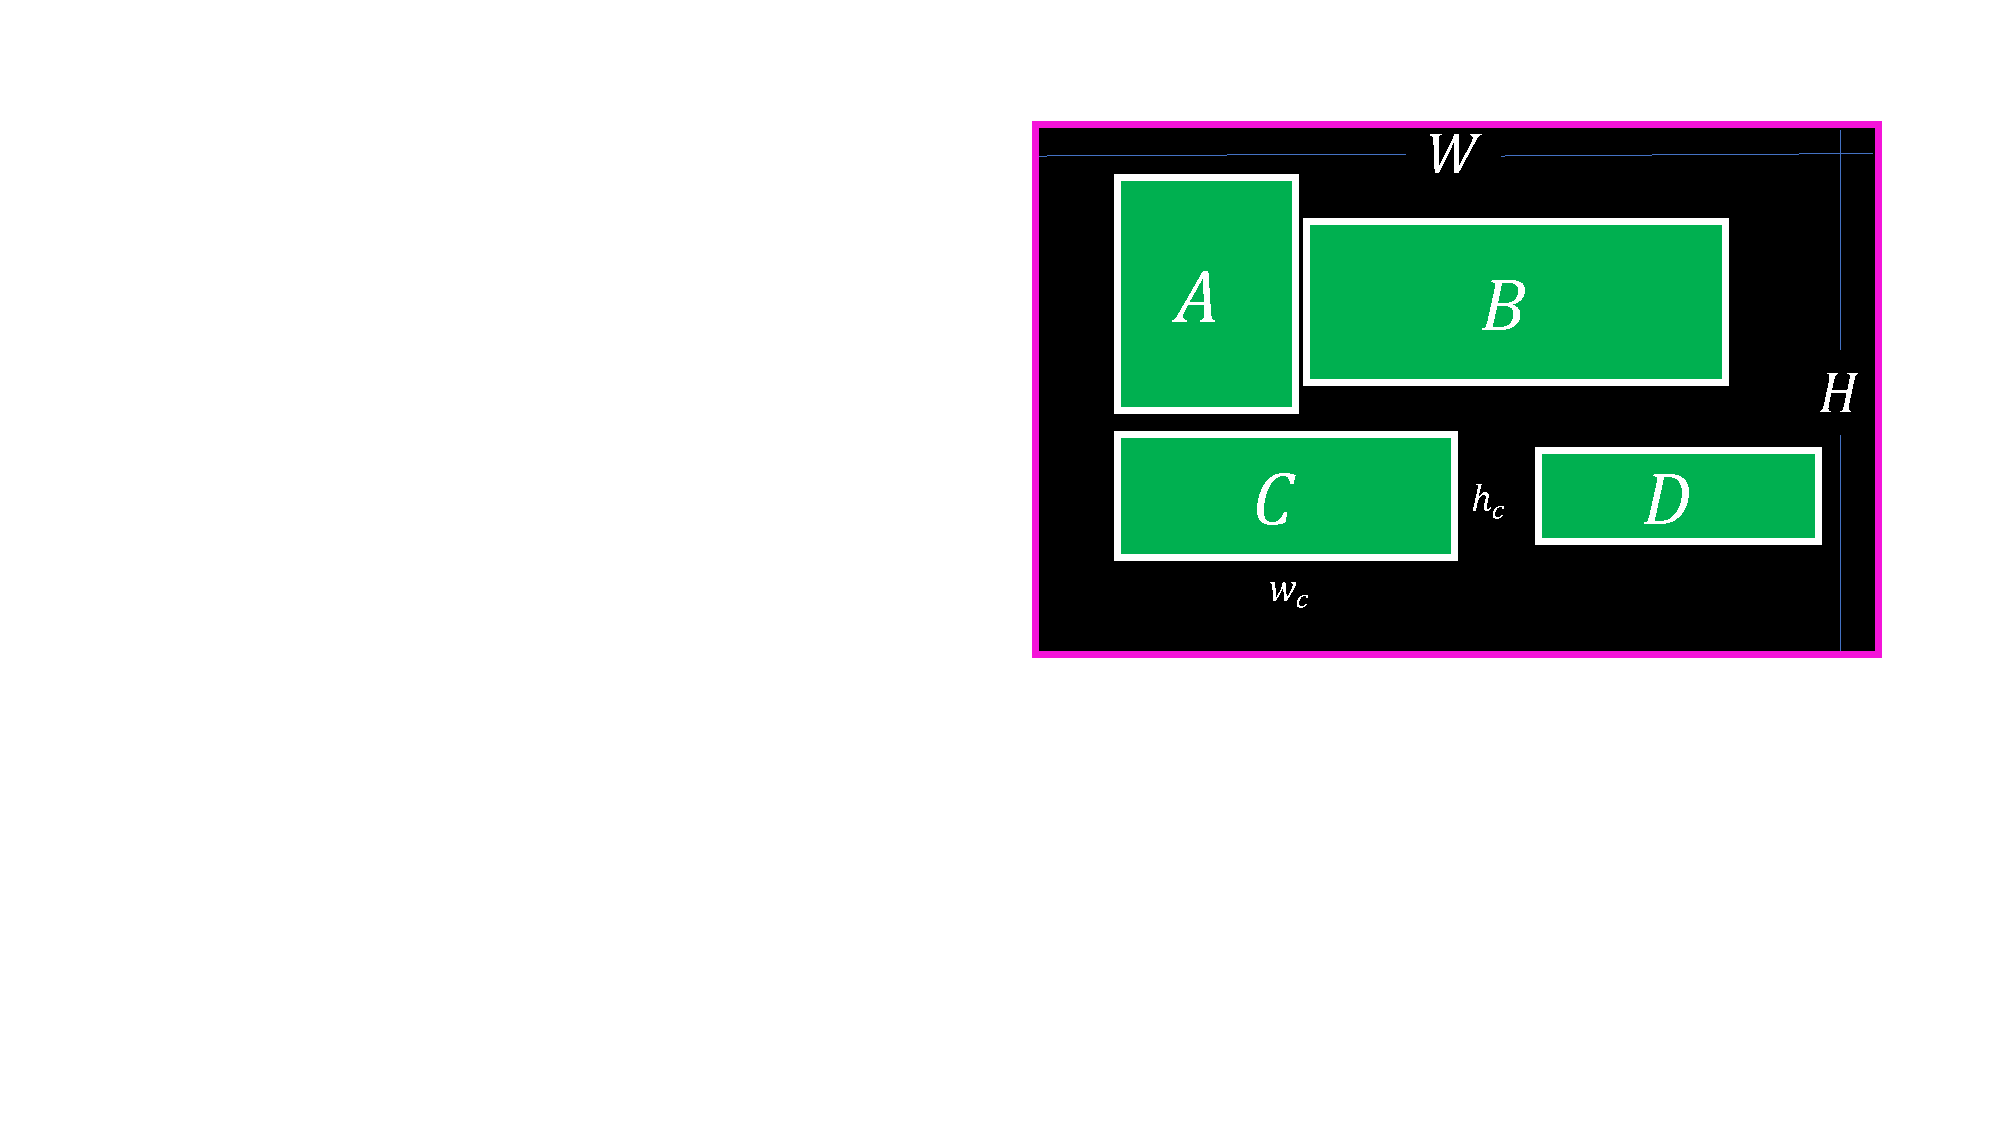
\includegraphics[width=0.4\textwidth]{config.pdf}}
   \caption{Illustrative configuration shows the relative position constraints for floor planning}
   \label{fig:config}
\end{figure}

\subsection*{Constraints}
We take here a different turn where we eliminate the relative position constraints. This is common in practice especially in VLSI design were the area of the building cells are known, however, the relative position is not known or not important. The makes the problem much harder since now there is no easy way to express the non-overlap conditions. Impose arbitrary relative positions constraints may lead to sub-optimal solution without good measure for how far the sub-optimal solution is from the optimal solution. Using brute-force won't scale well since the problem NP-hard~\citep{boyd2004convex}. 

To tackle this problem, we utilize a divide-and-conquer style algorithm to make the computation tractable. First, we divide the cells into two groups of two (almost-)equal areas based on their minimum area constraints. Second, one of the group is assigned to be left of all the cells of the other group and vice-versa. We do this recursively by diving each group into two sub-groups of (almost-)equal area and switch to assign the relative position as up-and-down. We keep iterating between direction of assignment until we reach an empty group. This can be seen as breadth-first search algorithm to construct $L$ and $U$ matrices.


%===========================================
\section{Results}
We implement the floor planning optimization problem without relative position constraints. Our implementation is done onto of CVX library in MATLAB. The code can be found under \url{https://github.com/Ahdhn/EEC254/blob/master/project/code/floor_planning.m}. Dividing the cells into (almost-)equal groups is a \emph{partition} problem for which we implemented a %greedy  algorithm that operates by sorting the input areas in ascending order. It then iterates over the sorted areas and assigns them to the group with least sum areas. 
heuristics algorithm that operates by randomize the area array and then iterates over randomized array and assigns the processed area to the group with least sum. The algorithm takes $O(nlog(n))$ where $n$ is the size of input area array. We compared our implementation using two models of 60 and 32 cells. The aspect ratio bounds are set to be between 0.5 and 2.0. We did our comparison against the solution given by Boyd et al.~\citep{boyd2004convex} as shown in Figure ~\ref{fig:comp}. Our solution have achieved better more tightly packed cells where the wasted area is $0\%$ and $1\%$ for the 32 and 60 cells respectively while Boyd et al. solution wasted area is $~38\%$ for both cases. 

\begin{figure}[!tbh]
\centering        
   \subfloat [Boyd - 60 Cells]{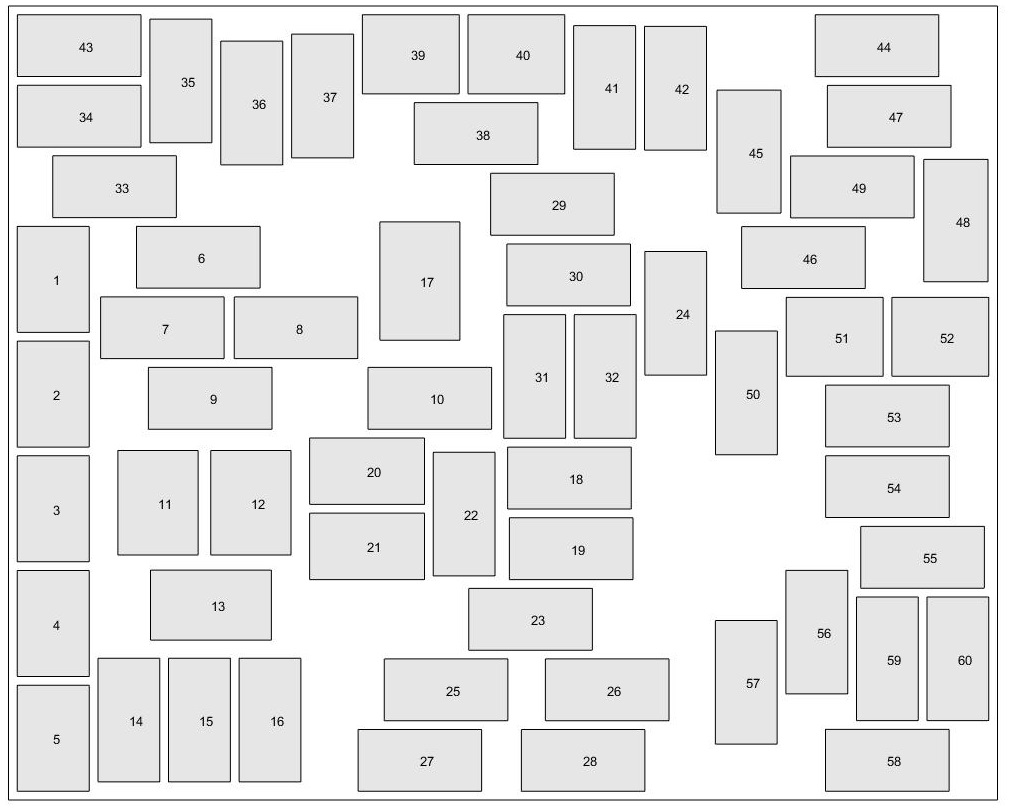
\includegraphics[width=0.25\textwidth]{boyd_60.jpg}}
   \subfloat [Boyd - 32 Cells]{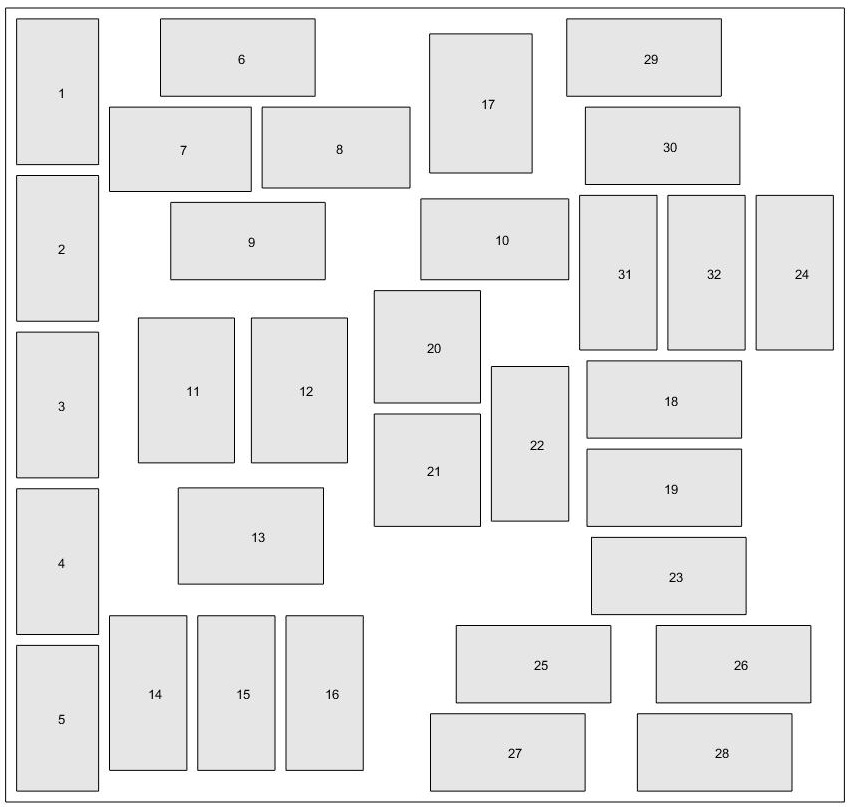
\includegraphics[width=0.25\textwidth]{boyd_32.jpg}}   
   \subfloat [Ours - 60 Cells]{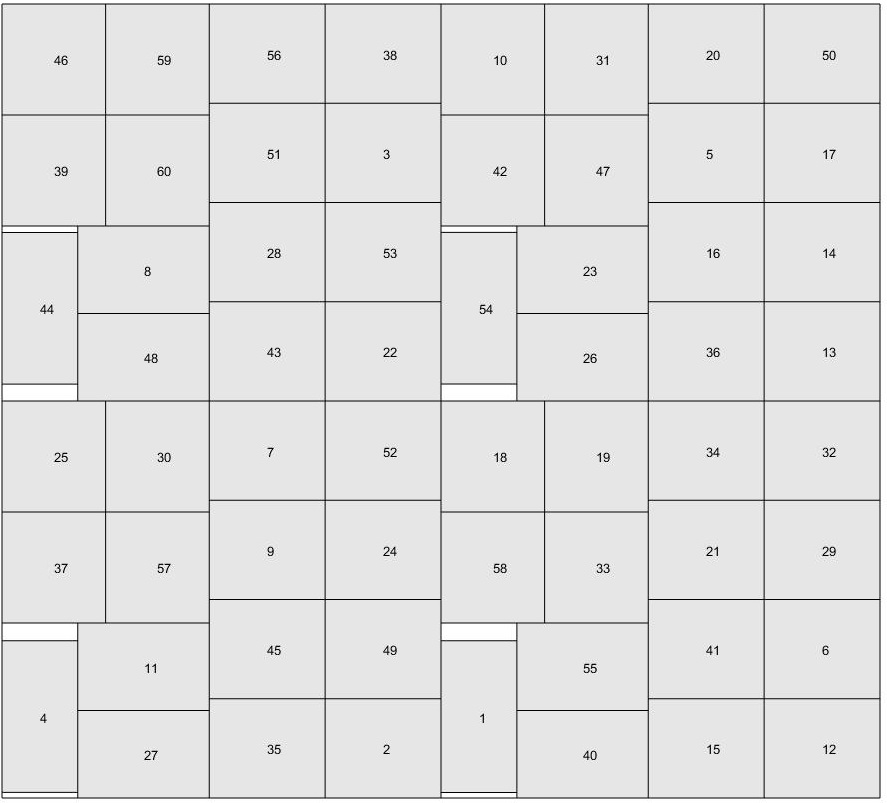
\includegraphics[width=0.25\textwidth]{our_60.jpg}}
   \subfloat [Ours - 32 Cells]{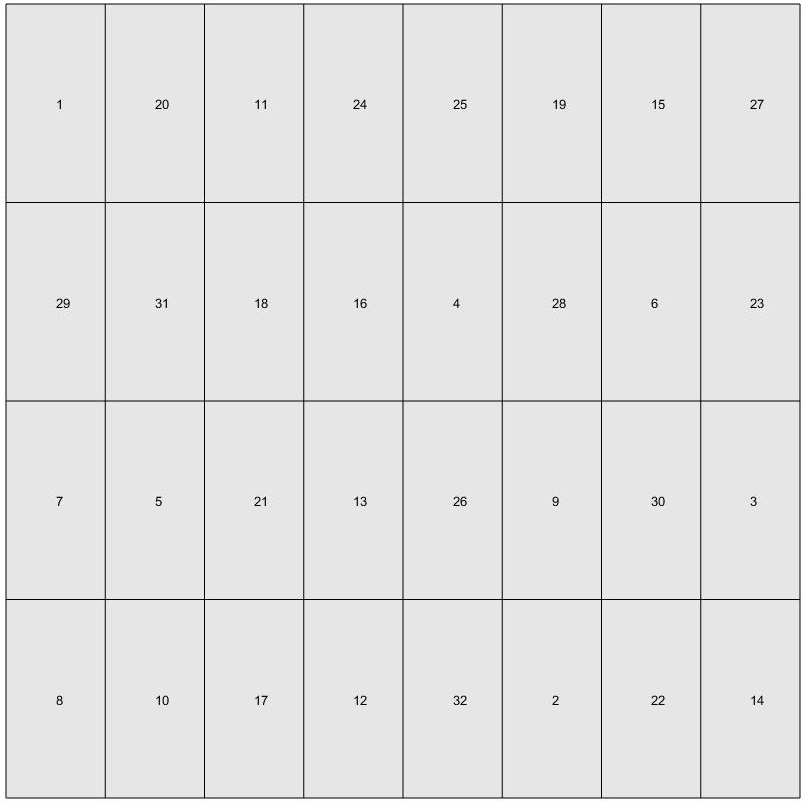
\includegraphics[width=0.25\textwidth]{our_32.jpg}}
   \caption{Comparison between our relative-positions-constraints-free model and Boyd et al.~\citep{boyd2004convex} solution for 60 and 32 cells.}
   \label{fig:comp}
\end{figure}



%===========================================
\section{Conclusion}
In this project, we showed the full formulation of the floor planning problem and how it can be solved as geometric programming problem while considering the majority of constraints taken into account in practice. Despite that we proposed to consider even more constraints, we found that considering less constraints is a problem that could happen more often in practice. We showed that it is better to have automated tool to assign the relative positions is better than assign them at random. 

\bibliography{mybib}
\end{document}
